\makeatletter
\def\input@path{{../../}}
\makeatother
\documentclass[../../main.tex]{subfiles}

\graphicspath{
	{../../img/}
	{../img/}
	{img/}
}

\begin{document}
\section{Независимость КрИ-2 от пути интегрирования}	

Говорят, что КрИ-2 $\displaystyle
\int\limits_{\tiny{\overbow{AB}}} P \, dx + Q \, dy$
не зависит от пути интегрирования, если он имеет одну и ту же 
величину для любой кривой с началом в точке $A$
и концом в точке $B$
(см. пример <<Физический смысл интегралов>> на стр. \pageref{indep-int}). 

Выражение
\begin{equation}
\label{lec_21, num_1}
P(x,y) \, dx + Q(x,y) \, dy
\end{equation} 
называют\emph{полным дифференциалом} в некоторой области $D$, если 
\[\exists F(x,y),\ (x,y) \in D : dF(x,y) = P(x,y) \, dx + Q(x,y) \, dy.\]
Функцию $F$ в этом случае называют \emph{первообразной} для \eqref{lec_21, 
num_1}.

\begin{thm}[основная теорема о КрИ] 
Пусть в односвязной области $D \subset \R^2$ определены функции $P$, $Q$,
непрерывные и имеющие непрерывные частные производные $P'_y$ и $Q'_x$.
Тогда следующие четыре условия равносильны: 

\begin{enumerate}[label=\arabic*$^{\,\circ}$]
	\item Для любого замкнутого кусочно-гладкого контура $L \subset D$ верно
	\[
	\ointctrclockwise\limits_{L} P(x,y) \, dx + Q(x,y) \, dy = 0; \]
	\item $\displaystyle\int\limits_{\tiny{\overbow{AB}}} P \, dx + Q \, dy$ не 
	зависит от пути интегрирования $\ \forall\, \overbow{AB} \subset D$;
	\item Выражение $P \,dx + Q \, dy$ является полным дифференциалом в $D$;
	\item В $D$ выполнены условия Эйлера: 
	\[ 
	P'_y(x,y) = Q'_x(x,y),\ \forall (x,y) \in D.
	\] 
	
\end{enumerate}
\begin{proof}
Доказательство проведём по следующей схеме: 

\[
1^{\circ} \implies 2^{\circ} \implies 3^{\circ} \implies
4^{\circ} \implies 1^{\circ}.
\]

\subsubsection*{$\mathbf{1^{\circ} \implies 2^{\circ}}$}

Пусть $A$ и $B$~--- любые две точки в области $D$, 
и I и II~--- пути между точками $A$ и $B$:

\begin{center}
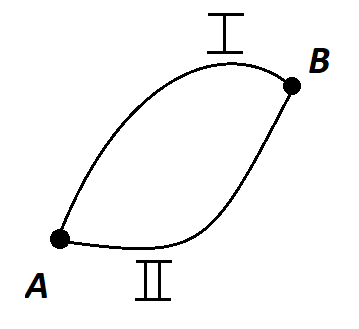
\includegraphics[scale = 0.5]{lec21_1.png}
\end{center}

Тогда контур $A_{I} B_{II}$~--- замкнутый. Значит,
\[
\int\limits_{\tiny{\overbow{A_I B_{II} A}}} P \, dx + Q \, dy = 0
\iff \int\limits_{\tiny{\overbow{A_I B}}} P \, dx + Q \, dy \ +
\int\limits_{\tiny{\overbow{B_{II} A}}} P \, dx + Q \, dy = 0 \iff \]
\[
\iff \int\limits_{\tiny{\overbow{A_I B}}} P \, dx + Q \, dy \ -
\int\limits_{\tiny{\overbow{A_{II} B}}} P \, dx + Q \, dy = 0
\implies \int\limits_{\tiny{\overbow{A_I B}}} P \, dx + Q \, dy \
= \int\limits_{\tiny{\overbow{A_{II} B}}} P \, dx + Q \, dy.
\]

\subsubsection*{$\mathbf{2^{\circ} \implies 3^{\circ}}$}

Зафиксируем какую-либо точку $M_0(x_0, y_0) \in D$. 
Тогда для $\forall M(x,y) \in D$ можно определить
$\displaystyle\int\limits_{\tiny{\overbow{M_0 M}}} P \, dx + Q \, dy = 
F(x,y)$. 
Он зависит только от точки $M_0$, т.~е. от $(x,y)$.

Покажем, что эта функция и является первообразной для \eqref{lec_21, num_1}:

\begin{center}
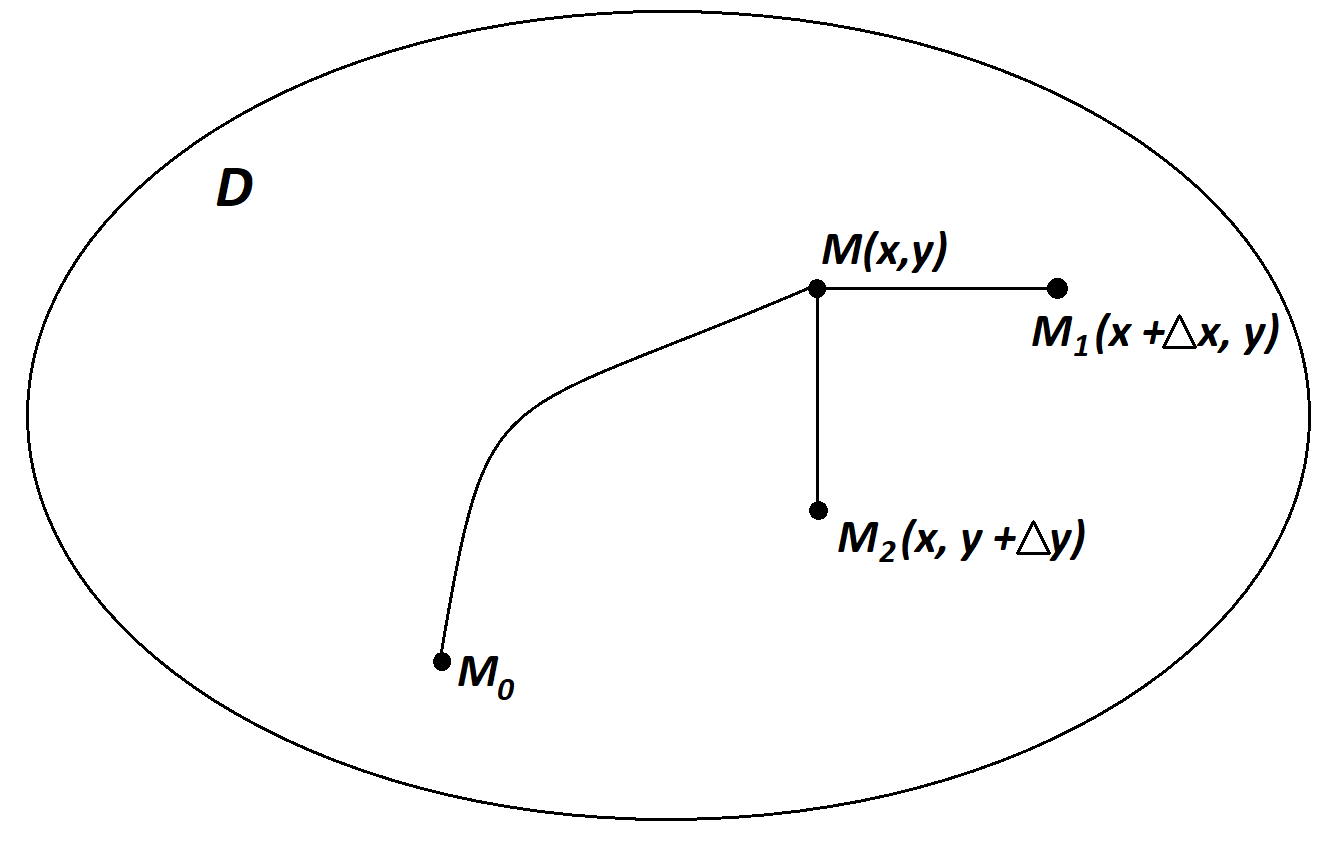
\includegraphics[scale = 0.35]{lec21_2.png}
\end{center}

Придаём приращение $\Delta x$ точке $M$, тогда
\[
\Delta_x F = F(x + \Delta x) - F(x) = 
\int\limits_{\tiny{\overbow{M_0 M_1}}} P \, dx + Q \, dy -
 \int\limits_{\tiny{\overbow{M_0 M}}} P \, dx + Q \, dy = *
\]
Будем считать, что кривая $M_0 M_1$ состоит из дуги
$\overbow{M_0 M}$ и отрезка $\overline{M M_1}$. Значит,
\[
* = \int\limits_{\overline{M M_1}} P(x,y) \, dx + Q(x,y) \, dy = \left[ 
\overline{M M_1}: 
\begin{cases} 
y = y = const, \\
x \in [x; x + \Delta x]
\end{cases}
\right] =
\int\limits_{x}^{x + \Delta x} P(x,y) \, dx = *
\]

Теорема о среднем:  
$\exists t \in [x; x + \Delta x] : * = P(t,y) \Delta x$, 
а тогда $\dfrac{\Delta F}{\Delta x} \appr{\Delta x \to 0} P(x,y)$, 
т.~е. $F'_x = P(x,y)$.

Аналогично, если мы придадим приращение $\Delta y$ точке $M$,
т.~е. получим точку $M_2(x, y + \Delta y)$, 
то, используя такие же рассуждения, получим $F'_y = Q(x,y)$.
А тогда 
\[
dF = F'_x \, dx + F'y \, dy  = P \, dx + Q \, dy,
\]
что и требовалось доказать.

\subsubsection*{$\mathbf{3^{\circ} \implies 4^{\circ}}$}

Имеем $P \, dx + Q \, dy = dF$, т.~е. $F'_x = P$, а $F'_y = Q$.

Тогда $F''_{xy} = P'_y,\ F''_{yx} = Q'_x \implies 
\left[  
\text{теорема о равенстве смешанных производных}
\right] 
\implies 
\implies P'_y = Q'_x$.

\subsubsection*{$\mathbf{4^{\circ} \implies 1^{\circ}}$}

Возьмём гладкий контур $L \subset D$. 
Пусть он ограничивает область $G \subset D$, тогда по формуле Грина

\[
\ointctrclockwise\limits_{L} P \, dx + Q \, dy = 
\iint\limits_{G} (Q'_x - P'_y)\, dx\, dy = 
\iint\limits_{G} 0\, dx\, dy = 0.
\qedhere
\]
\end{proof}
\end{thm}

\section{Вычисление первообразной}

Пусть в области $D$ выполнены условия Эйлера. 
Значит, существует первообразная для $P \, dx + Q \, dy$:
\[F(x,y) = \int\limits_{(x_0,y_0)}^{(x,y)} P \, dx + Q \, dy.\]

Здесь
интеграл не зависит от пути интегрирования. 
В таких случаях интеграл
\[\displaystyle\int\limits_{\tiny{\overbow{AB}}} P \, dx + Q \, dy\] принято 
записывать
\[\displaystyle\int\limits_{A}^{B} P \, dx + Q \, dy.\]

В простейших случаях функцию $F(x,y)$ можно найти так:
\begin{center}
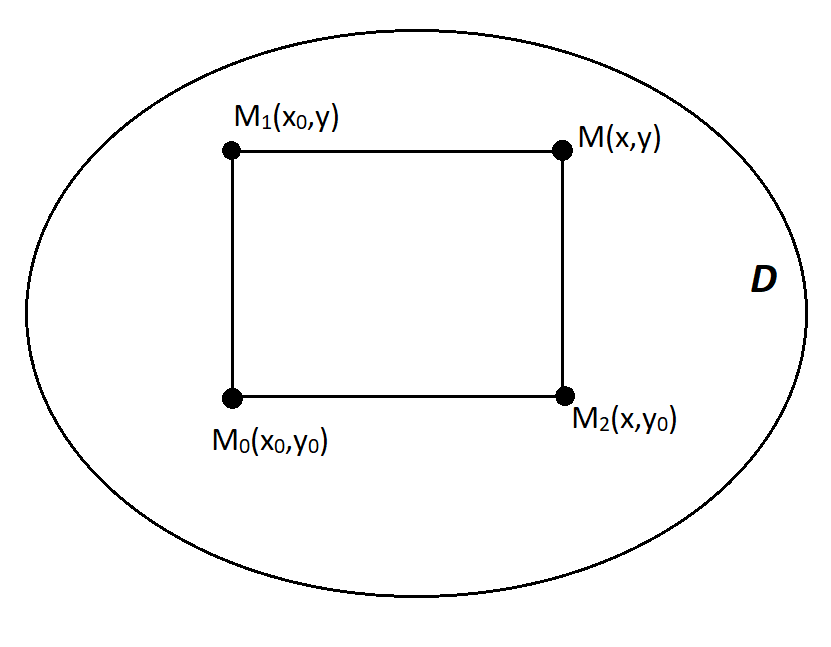
\includegraphics[scale = 0.5]{lec21_3.png}
\end{center}
\[
F(x,y) = \int\limits_{\overline{M_0 M_1}} P \, dx + Q \, dy \ +
\int\limits_{\overline{M_1 M}} P \, dx + Q \, dy
= *
\]

В первом интеграле $x = const,\, dx = 0,\ y \in [y_0; y]$.
Во втором~--- $y = const,\, dy = 0,\ x \in [x_0;x]$. Тогда:
\[
* = \int\limits_{y_0}^{y} Q(x_0, y) \, dy +
\int\limits_{x_0}^{x} P(x,y) \, dx.
\]

Таким образом,
\[
F(x,y) = \int\limits_{x_0}^{x} P(x,y) \, dx +
\int\limits_{y_0}^{y} Q(x_0, y) \, dy.
\]

Здесь $(x_0,y_0)$~--- любая точка области.

Если в качестве кривой $\overbow{M_0 M}$ взять $\overbow{M_0 M_2 M}$, то 
получим 
\[
F(x,y) = \int\limits_{y_0}^{y} Q(x, y) \, dy +
\int\limits_{x_0}^{x} P(x,y_0) \, dx.
\]

\section{Использование первообразной для вычисления интегралов}

Пусть в $D$ выполнены условия Эйлера и рассматривается интеграл

\[
\int\limits_{\tiny{\overbow{AB}}} P(x,y) \, dx + Q(x,y) \, dy = *
\]

Заменим $\overbow{AB}$, если необходимо, гладкой кривой
$
\begin{cases} x = x(t), 
\\ y = y(t), 
\\ \alpha \leq t \leq \beta,
\end{cases}$
у которой \\
$
\begin{cases} 
(x(\alpha), y(\alpha)) \longleftrightarrow A, \\
(x(\beta), y(\beta)) \longleftrightarrow B,
\end{cases}
$ тогда
\[
* = 
\int\limits_{\alpha}^{\beta}(
P(x(t), y(t)) \cdot x'(t) +
Q(x(t), y(t)) \cdot y'(t)
) \ dt = 
\int\limits_{\alpha}^{\beta} F'_t(x(t), y(t)) \ dt =
F(x(t), y(t)) \bigg|_{\alpha}^{\beta} =
\]
\[
= F(x(\beta), y(\beta)) - F(x(\alpha), y(\alpha)) = 
F(x,y) \bigg|_A^B.
\] 

То есть,
\[\int\limits_{\tiny{\overbow{AB}}} P \  dx + Q \, dy =
F(x,y) \bigg|_A^B.\]

\begin{example}
\begin{gather*} 
I = \int\limits_{\tiny{\overbow{AB}}} 2xy \, dx + x^2 \, dy, \\
A(1,0),\ B(10,2).
\end{gather*}

\[P'_y = 2x,\ Q'_y = 2x.\]

Выполнены условия Эйлера. Найдём первообразную:
\[
F(x,y) = \int\limits_{x_0}^{x} P(x,y) \, dx\ +
\int\limits_{y_0}^{y} Q(x_0, y) \, dy = 
\left[ 
(x_0,y_0) = (0,0)  
\right] =
\int\limits_{0}^{x} 2xy \, dx\ + 
\int\limits_{0}^{y} 0 \, dy = 
\int\limits_{0}^{x} 2xy \, dx = 
x^2y.
\]
\[
I = x^2y \bigg|_{(1,0)}^{(10,2)} = 200.
\]
\end{example}
\end{document}
